% A LaTeX (non-official) template for ENSI projects reports
% Copyright (C) 2025 ENSI


\documentclass[12pt,a4paper]{report}

% Encodage et langues
\usepackage[utf8]{inputenc}  % Encodage UTF-8 (obsolète mais utile pour pdflatex)
\usepackage[T1]{fontenc}     % Encodage des fontes
\usepackage[french]{babel}  % Langue principale du document
%\usepackage[english]{babel}  % Décommentez si vous écrivez en anglais

% Mappages Unicode nécessaires en mode pdfLaTeX (translittération)
\DeclareUnicodeCharacter{1E24}{\d{H}}
\DeclareUnicodeCharacter{1E63}{\d{s}}
\DeclareUnicodeCharacter{0100}{\=A}
\DeclareUnicodeCharacter{0101}{\=a}
\DeclareUnicodeCharacter{016B}{\=u}

% Mise en page et marges
\usepackage{geometry}        % Configuration des marges
\geometry{a4paper, margin=2.5cm}

% Gestion des titres et en-têtes/pieds de page
\usepackage{titlesec}        % Personnalisation des titres
\titleformat{\chapter}[frame]{\normalfont\huge\bfseries}{\chaptername\ \thechapter}{20pt}{\Huge}
\usepackage{fancyhdr}        % Personnalisation des en-têtes et pieds de page
\pagestyle{fancy}
\renewcommand{\chaptermark}[1]{\markboth{#1}{#1}}
\fancyhead[R]{\thepage}
\fancyhead[L]{\chaptername\ \thechapter\ --\ \leftmark}

% Mathématiques
\usepackage{amsmath, amssymb, amsthm, bm}

% Algorithmes
\usepackage{algorithm}
\usepackage{algpseudocode}
%\usepackage{listofalgorithms} % Pour générer la liste des algorithmes

% Gestion des images et figures
\usepackage{graphicx}        % Inclusion d'images
\graphicspath{{images/}}     % Chemin par défaut des images
\usepackage{subfig}          % Sous-figures
\usepackage{float}           % Positionnement exact des figures

\usepackage{multirow}
\usepackage{longtable}
\usepackage[table]{xcolor}
\usepackage{float}

% Tableaux et mises en page avancées
\usepackage{array, multirow} 

% Gestion des références et bibliographies
\usepackage{hyperref}        % Liens cliquables dans le PDF
\usepackage[footnote]{acronym} % Acronymes en note de bas de page
\usepackage[resetlabels,labeled]{multibib} % Bibliographies multiples
\newcites{URL}{Netographie}  % Bibliographie spécifique aux sources Internet
\usepackage{url}            % Formatage des URL

% Texte en arabe (pour pdflatex uniquement)
% \usepackage{arabtex}         % Texte arabe
% \usepackage{utf8}            % Assurer la compatibilité UTF-8

% Gestion des sous-fichiers
\usepackage{subfiles}

% Définition de tailles pour figures
\newlength\figureheight
\newlength\figurewidth
% si le rapport est écrit en français
\renewcommand{\listalgorithmname}{Liste des Algorithmes} % Mettre en commentaire en cas de rapport en anglais
% Insertition de fichier pdf
\usepackage{pdfpages}
\usepackage{lettrine}

\begin{document}

%%%%%%%%%%%%%%%%%%
%%% Page de garde %%%
%%%%%%%%%%%%%%%%%%

\subfile{pg-ENSI} 
%\subfile{pg-ENSI_ang} % if english report
\clearpage
%%%%%%%%%%%%%%%%%%%%%%%%%%%%%%%%%%%%%%%%%%%%%%%%%%%%%%%%%%
    %%% Remerciements, tables de matières, etc %%%
%%%%%%%%%%%%%%%%%%%%%%%%%%%%%%%%%%%%%%%%%%%%%%%%%%%%%%%%%%

%\frontmatter

\clearpage
\subfile{0-i-signature}
\clearpage
% Insérer le résumé

% Écrire votre résumé en trois langues dans le fichier Résumé.docx.
% Convertir Resume.docx en Resume.pdf.

% Ajouter le fichier dans main.tex :

\clearpage
\pagenumbering{roman}
\subfile{0-iii-Remerciements}
\clearpage
% Insérer le résumé

% Écrire votre résumé en trois langues dans le fichier Résumé.docx.
% Convertir Resume.docx en Resume.pdf.

% Ajouter le fichier dans main.tex :
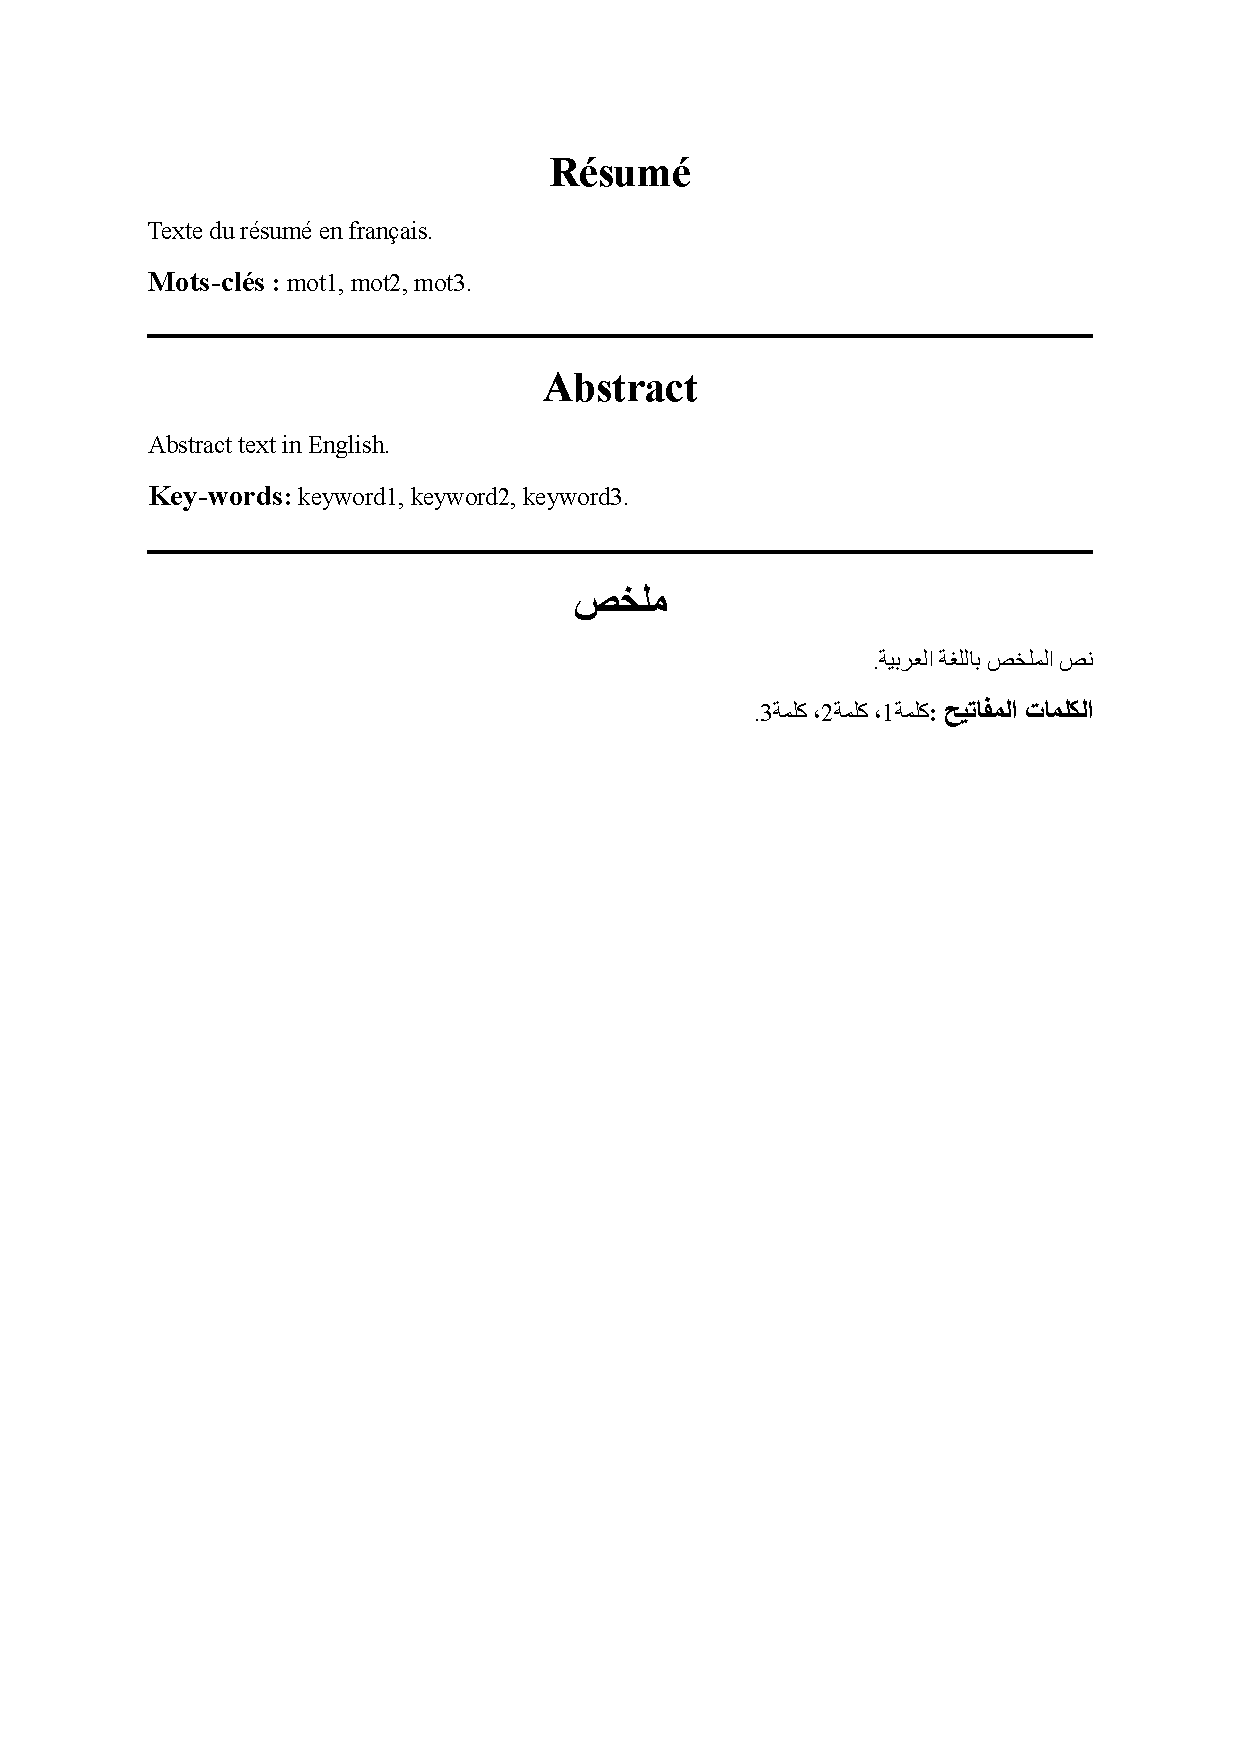
\includepdf[pages=-]{Resume.pdf}
\clearpage

\clearpage
\tableofcontents
\clearpage
\listoffigures
\clearpage
\listoftables
\clearpage
\clearpage
%\chapter*{Liste des acronymes}
\chapter*{List of acronyms}% if english report
\begin{acronym}[ACRO5] % Give the longest acronym here
\acro{ACRO1}{\emph{ACRONYME1}}
\acro{ACRO2}{\emph{ACRONYME2}}
\acro{ACRO3}{\emph{ACRONYME3}}
\acro{ACRO4}{\emph{ACRONYME4}}
\acro{ACRO5}{\emph{ACRONYME5}}
\end{acronym}





%%%%%%%%%%%%%%%%%%%%%%%%%%%%%%%%%%%%%%%%%%%%
%%% Corps du rapport et les références %%%
%%%%%%%%%%%%%%%%%%%%%%%%%%%%%%%%%%%%%%%%%%%%


\pagestyle{fancy}

\cleardoublepage
\pagenumbering{arabic}
\subfile{0-introduction}
\subfile{1-first-chapter}
\subfile{2-chapter}
\subfile{3-chapter}
\subfile{4-chapter}
\subfile{2-conclusion}
\subfile{Bibliographie.tex}






\section*{Netographie}

% Définition du compteur customref
\newcounter{customref}

\begin{itemize}
    \refstepcounter{customref} % incrémente le compteur
    \item[\hypertarget{refTalanTunisie}{\textbf{[\thecustomref]}}] 
    Talan Tunisie, Adresse : \href{https://www.linkedin.com/company/talan-tunisie/about/}{https://www.linkedin.com/company/talan-tunisie/about/}

    % Momentic AI
\refstepcounter{customref}
\item[\hypertarget{ref\thecustomref}{\textbf{[\thecustomref]}}]
\label{ref:MomenticAI}
Momentic AI, plateforme SaaS pour tests fonctionnels automatisés, consultable sur : 
\href{https://momentic.ai/}{https://momentic.ai}

% Blok AI
\refstepcounter{customref}
\item[\hypertarget{ref\thecustomref}{\textbf{[\thecustomref]}}]
\label{ref:BlokAI}
Blok AI, outil SaaS pour validation UX et détection d’anomalies visuelles : 
\href{https://www.joinblok.co/}{https://www.joinblok.co/}

% Browser-Use
\refstepcounter{customref}
\item[\hypertarget{ref\thecustomref}{\textbf{[\thecustomref]}}]
\label{ref:BrowserUse}
Browser-Use, bibliothèque open source pour navigation web autonome par LLM : 
\href{https://github.com/browser-use/browser-use}{https://github.com/browser-use/browser-use}

% ThunderCode
\refstepcounter{customref}
\item[\hypertarget{ref\thecustomref}{\textbf{[\thecustomref]}}]
\label{ref:ThunderCode}
ThunderCode, plateforme SaaS de génération de tests IA et personas autonomes : 
\href{https://www.thunders.ai/}{https://www.thunders.ai/}

% UXAgent
\refstepcounter{customref}
\item[\hypertarget{ref\thecustomref}{\textbf{[\thecustomref]}}]
\label{ref:UXAgent}
UXAgent, article de recherche sur la simulation de comportements utilisateurs : 
\href{https://arxiv.org/abs/XXXX.XXXXX}{https://arxiv.org/abs/XXXX.XXXXX}

% Méthodologie Scrum
\refstepcounter{customref}
\item[\hypertarget{ref:AgileScrum}{\textbf{[\thecustomref]}}]
\label{ref:AgileScrum}
Méthodologie Agile Scrum, consultable sur : 
\href{https://toolapp.fr/methode-agile-scrum/}{https://toolapp.fr/methode-agile-scrum/}


% Scrum
\refstepcounter{customref}
\item[\hypertarget{ref\thecustomref}{\textbf{[\thecustomref]}}]
\label{ref:Scrum}
ToolApp, Méthode agile Scrum : 
\href{https://toolapp.fr/methode-agile-scrum/}{https://toolapp.fr/methode-agile-scrum/}

\end{itemize}



\end{document} 